\documentclass[12pt]{article}
\usepackage[margin=1in]{geometry}
\usepackage[english]{babel}
\usepackage[utf8x]{inputenc}
%% \usepackage[rm,light]{roboto}
%% \usepackage[T1]{fontenc}
\usepackage{quattrocento}
\usepackage[T1]{fontenc}
\usepackage{amsmath}
\usepackage{graphicx}
\usepackage{indentfirst}
\usepackage{float}
\usepackage{url}
\usepackage{caption}
\usepackage[toc,page]{appendix}
\usepackage{tocloft}
\usepackage{xcolor}
\usepackage{hyperref}
\usepackage{longtable}
\hypersetup{
  colorlinks = true,
  linkcolor = [rgb]{0,0,0.5},
  urlcolor = [rgb]{0,0,0.5}
}

\graphicspath{ {./images/} }
\renewcommand\cftaftertoctitle{\par\noindent\hrulefill\par\vskip-0.5em}

\begin{document}

\begin{titlepage}

  \newcommand{\HRule}{\rule{\linewidth}{0.5mm}} % Defines a new command for the horizontal lines, change thickness here
  
  \topskip0pt
  \vspace*{\fill}
  \center % Center everything on the page
  
  { \huge \bfseries Magic Drawing}\\
  \HRule \\[1cm]

  \large Blaze Kotsenburg\\
  \large Jake Maschoff\\
  \large Raj Patel\\[1cm]
  
  \normalsize \today\\[4cm]
  
  
\includegraphics[width=0.30\textwidth]{logo.png}
  \vspace*{\fill}
  
\end{titlepage}

\newpage
\tableofcontents
\noindent\hrulefill
\newpage

\begin{abstract}
  \addcontentsline{toc}{section}{Abstract}
  
  Today, we find ourselves surrounded by a multitude of electronics and technologies. We use these technologies for our entertainment, exploration, science, and research. When our team looked at the fields that technology is used for, we saw many great innovations and use cases that involved electronics. We discovered that there are many great ways in which electronics can be integrated into art pieces while doing our research for project ideas. Art does not need the integration of technology, but it allows for a whole new realm of innovations and creativity. Our objective is to create an art piece that combines both Computer and Mechanical Engineering. We want to build a visual art display consisting of LED’s and motors on linear tracks. Our goal is to have users interact with our art piece and in return, the user will be immersed in a visual light show.
\end{abstract}

\section{Introduction}
When we were deciding on a project, we wanted to do a project which would use our computer engineering knowledge to its fullest. Initially, we decided to create a more advanced and up-to-date avalanche beacon. However, we ran into many conflicts with the antenna for backwards compatibility and due to internships over the summer, the team wasn’t able to meet as we had planned. Thus, we were afraid the project would not get done in time. As a result, we decided that it would be best if we chose a project that we were more passionate about and could be accomplished within our given time frame. 

When doing research for a new project, we wanted to choose a project that would improve something that already existed or design something new that would solve a problem. However, after extensive research we couldn’t settle on anything. After seeking help, our project advisor suggested that we do an art piece. Excitingly, all of us agreed on doing an art piece and we wanted it to be big and complex. 

Ultimately, we decided on an art piece that depicted a painting canvas. There are two main components of this project: an iOS app and a 3D LED canvas. A user can draw something with the iOS app, which is then displayed on the 3D LED canvas with different effects. The LED canvas consists of many LED strips and a mechanical X, Y, and Z coordinate linear track system behind it. Basically, the linear track system acts as the user’s finger on the iOS app. Wherever the user is drawing, the linear track will follow the user’s finger in the X and Y direction while protruding the LED strips out in the Z direction with an actuator to create a 3D effect. 

Although the art piece does not necessarily solve a problem, it does use skills we’ve learned throughout our Computer Engineering academic career. With our art project, we hope to inspire people and show how engineering can be used as a form of art.

\section{Background}
Once we had decided to do an art project, we began doing research into existing art pieces that involve engineering. We discovered the  Coca Cola display in Time Square while searching for projects. It is a visual display that combines mechanical and computer engineering. The display itself is used for marketing purposes but shows that the combination engineering and art can be used to make very expressive designs. As seen in Fig. \ref{fig:cocacola}, the Coca Cola display creates a 3D effect using LED blocks (similar to a 64x64 LED block) with actuators attached behind them. The actuators move the blocks in and out of the display at different sequences to showcase a visual art show.

\begin{figure}[H]
  \centering
  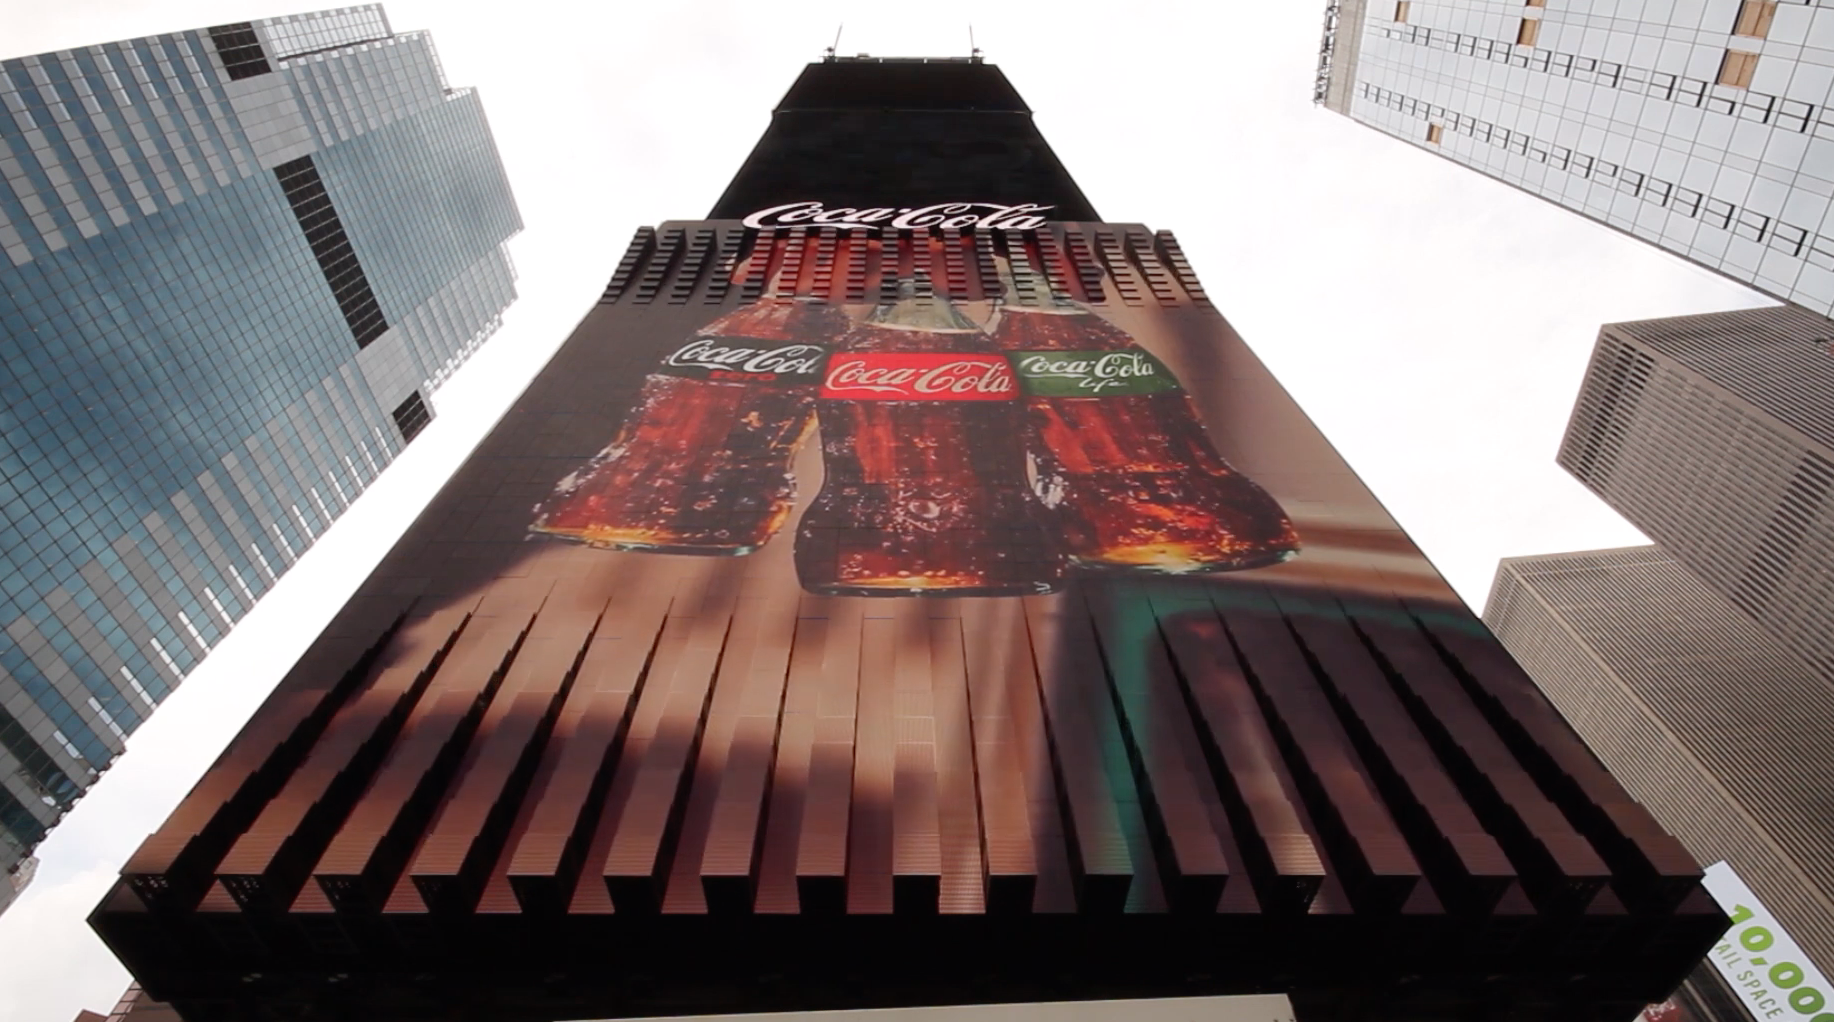
\includegraphics[width=1\textwidth]{image1.png}
  \caption{Coca Cola Time Square Display creating a 3D effect via actuators and LEDs.}
  \label{fig:cocacola}
\end{figure}

Originally, we wanted to create a 3D display similar to Fig. \ref{fig:cocacola}. However, in order to make our project significant, this would have required a large amount of 64x64 LED blocks and actuators, which are both rather expensive and out of our budget. As a result, we started to think about a cheaper alternative for a 3D display. Instead of LED blocks with actuators behind each block, we decided to use LED strips, linear tracks, and motors to move a single actuator through a 2D space. The actuator then applies pressure to the back of the canvas, giving the Canvas a 3D effect. Our linear tracks are inspired by CNC and 3D printers because they move very smoothly with high precision which is what we wanted.

\section{Implementation}
Once we had our idea for the project in place, we started designing the art piece. As we mentioned earlier, we want our art piece to be large and significant. We started doing research to figure out the combinations of parts that could maximize the size of the project. After extensive research, we settled on a dimension of 1m x 2m for the 3D canvas.

\begin{figure}[H]
  \centering
  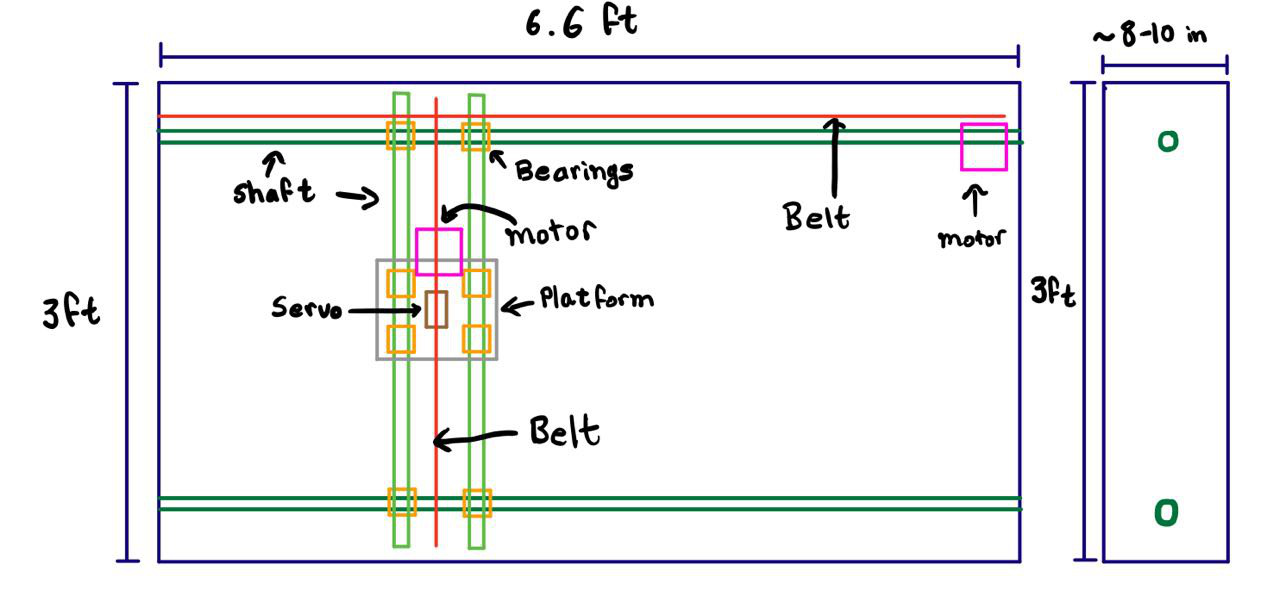
\includegraphics[width=0.9\textwidth]{image4.png}
  \caption{Design of 3D canvas with its components in place.}
  \label{fig:design}
\end{figure}

In our initial planning phase, we started off by designing the frame to house parts related to linear track systems. Fig \ref{fig:design}. shows the placements of the parts in the 1m x 2m frame. The art piece consists of six key components: LEDs, a linear track system, an iOS app, microcontroller firmware, and an actual frame for housing all of the devices.

\subsection{LEDs}
For our canvas we wanted LED strips that were capable of RGB and could be individually indexable. After doing research, we found Adafruit NeoPixel Digital RGB LED Strips to be the best option. There were many benefits in using these LED strips that went into our decision. First and foremost, the Adafruit LED strips are capable of RGB and each LED on the strip can be indexed individually, which is exactly what we were looking for. These LED strips are 2m long, which is a good length to make a fairly large display. By placing 18 LED strips 1 ½ inches apart, we were able to get an adequately sized display. With 18 2m long LED strips placed 1 ½ inches apart, the final dimension of the display is 1m x 2m. Fig. \ref{fig:ledstripsonsheet} shows the LED strips spaced out by 1 ½ inches and taped down to a normal bed sheet.

\begin{figure}[H]
  \centering
  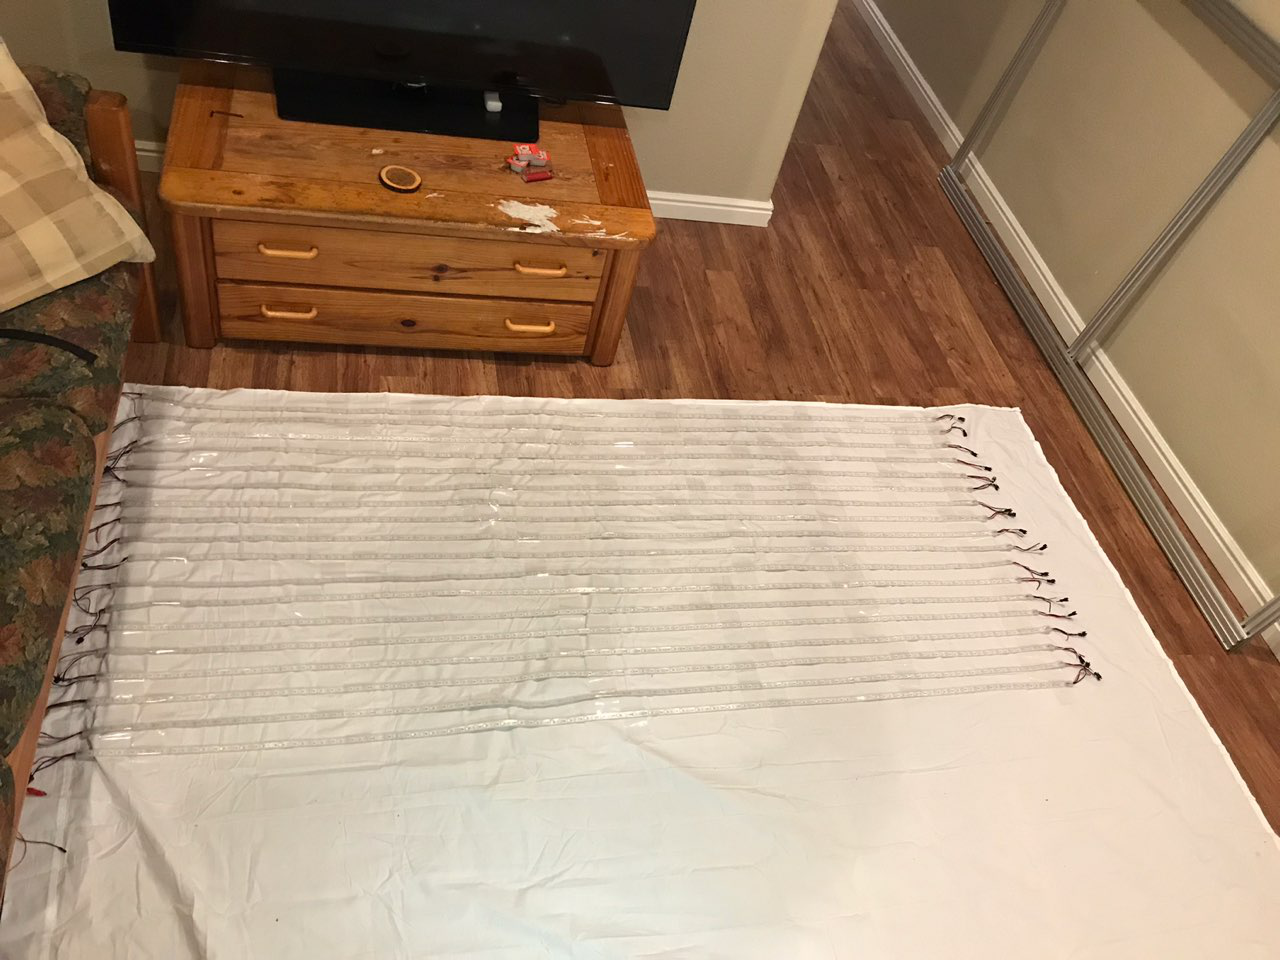
\includegraphics[width=0.7\textwidth]{image6.png}
  \caption{Canvas made out of 18 LED strips.}
  \label{fig:ledstripsonsheet}
\end{figure}

One of the other major benefits was Adafruit’s open source library for the LED strips. Their library gives us full control of the LED strips. We can easily index each LED pixel on the strip to control the brightness and the color. Each pixel’s color can be set by using RGB values.

\subsection{Linear Track System}
Once the LED strips were picked out, we needed linear tracks that could span the dimension of the display. However, none of us have any background in mechanical engineering, which resulted in us to do thorough research before we purchased anything. In our research we encountered aluminum linear rails, T-slot aluminum extrusions, and V-slot aluminum extrusions. After going back and forth with these three options, we ultimately decided on selecting the V-slot aluminum extrusions. The V-slot extrusions allows for ease of movement via wheels, pulley, timing belt, and stepper motors. 

With no background in linear motion, we were not sure of the amount of torque we needed in order to move the actuator around the 2D plane. Thus, we decided it would be of our best interest if we purchased a couple of high torque stepper motors. After settling on the motors, we purchased an appropriate pulley, a timing belt, and a power supply.

Now, we needed a way to drive these motors. We originally planned on designing our own motor drivers. However, that plan was derailed as we had a late start on the project and we still needed a lot of planning to be done in order to design our own PCBs for the motor drivers. Thus, we decided to purchase Pololu AMIS-30543 Stepper Motor Driver. This motor driver is capable of delivering 3A, which is what the motor needs to be effective. 

The last part we needed for the linear track system was an actuator. The actuator needed to extend out far enough for the user to see the 3D effect. We ended up purchasing a mini actuator capable of extending out to 3 inches.

\begin{figure}[H]
  \centering
  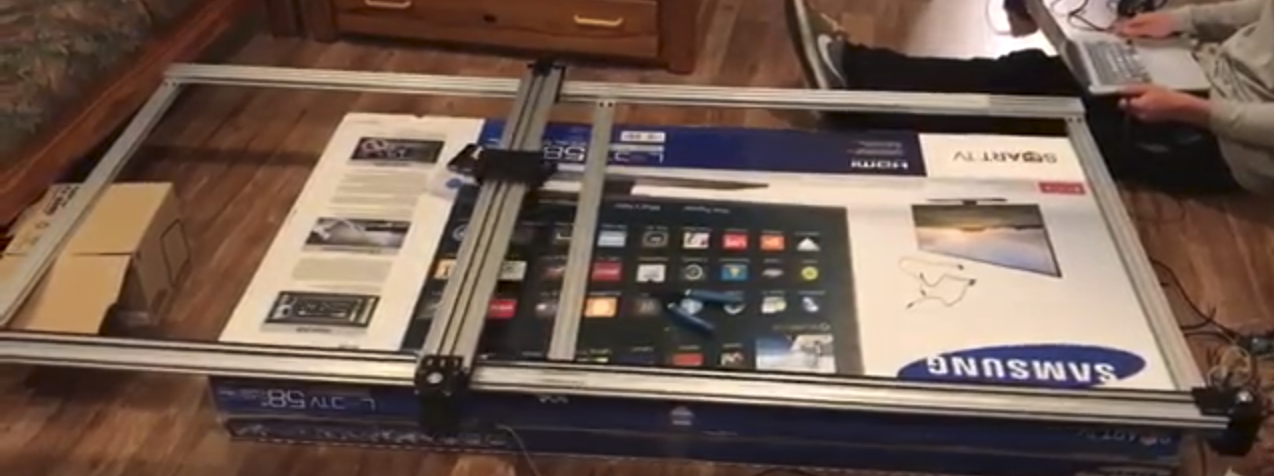
\includegraphics[width=0.85\textwidth]{image2.png}
  \caption{Assembled extrusions, stepper motors, timing belts, pulleys, and gantry cart to create a 2D plane.}
  \label{fig:lineartracks}
\end{figure}

Assembling the extrusions was fairly straight forward, however, we did encounter a few problems. We could not find a 2m long extrusion for X-axis, so we decided to connect two 1m extrusions together. We also needed a way to support the two X-axis rails to prevent them from moving. To do this, we attached three 1m extrusions on the back, one on each end, and one on the center. The 1m support extrusions behind the 2m X-axis extrusions can be seen in Fig. \ref{fig:lineartracks}.

After assembling the base of our 2D plane, we started to install the stepper motors, timing belts, pulleys and the gantry carts. The motors are installed on one end of the extrusion while the pulleys are installed on the opposite end. The ends of the timing belt attach to the gantry cart while the rest of the belt loops around the stepper motor and the pulley. The complete assembly is pictured in Fig. \ref{fig:lineartracks}.

\subsection{Mobile iOS App}
The biggest part of our project requires the art piece to be interactive with the user. In order to make this happen, we chose to design a mobile application for iOS that will communicate with the LED Canvas directly. The app is developed in Swift, which is the language that has begun to take place of Objective-C. Swift is developed by Apple specifically for Apple products. We already have a iPad to use for demo day so this made the most sense for us.

The application uses a Bluetooth framework provided by Swift called CoreBluetooth framework for communicating to the board. The framework has protocols that are required to be implemented for communicating to any Bluetooth device. It was in our best interest to make sure that we are communicating with the correct Bluetooth chip so the main view will populate a table of available Bluetooth chips to connect to. The app will search for available devices and then populate the table allowing the user to select the desired chip to connect to.

\begin{figure}[H]
  \centering
  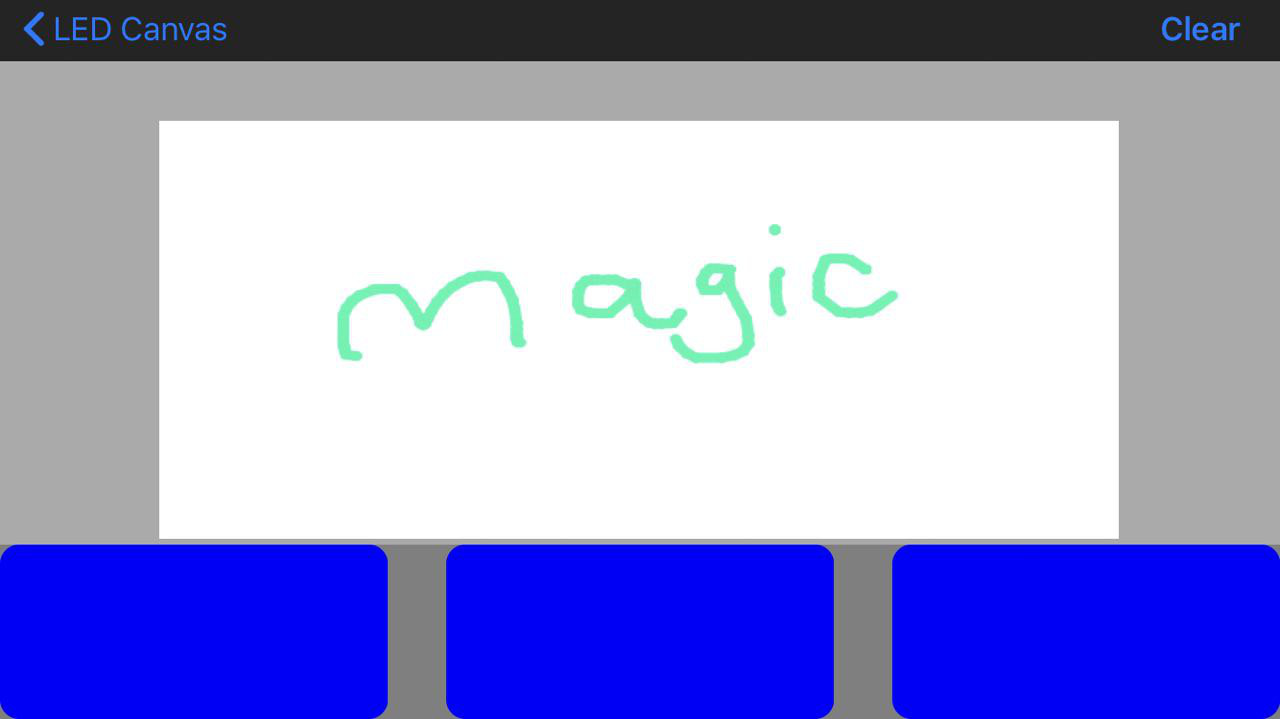
\includegraphics[width=0.75\textwidth]{image3.png}
  \caption{A screenshot of our app in development. The blue rectangles represent buttons that will give users more control.}
  \label{fig:iosapp}
\end{figure}

Once the chip is selected for connection (i.e. the LED Canvas), the application presents a new screen to the user that enables them to draw as seen in Fig. \ref{fig:iosapp}. The user can select the color of the LED’s, a filter for the brush, and light show patterns to display that are built into the software on the Arduino side. When a user draws on the app, whatever they are drawing begins to fade away. This makes it more of a tracing application in which the motors and lights follow on the LED Canvas.

The drawing portion of the application uses the CoreGraphics framework powered by Quartz technology (drawing engine) to render 2D graphics to the view. This framework provides tools and an environment to draw in, making the implementation straight forward and precise.

\subsection{Microcontroller Firmware}
Another one of our main components for this art project is a way of controlling the LEDs, motors, and communicating with the mobile iOS app. Since there are many devices, we needed a microcontroller that had a large number of I/O pins. We purchased an Arduino Mega which has more than the needed number of I/O pins. The arduino will have all of the 18 LEDs, 2 motor drivers, and Bluetooth device connected to it.

For the actual code, we wanted to keep things clean and well documented. This meant creating separate classes/modules for each of the components connected to the arduino. We created a class for controlling the LEDs. This class keeps track of all 18 LED strips. We implemented various functions to control each pixel individually. Based on the user input from the iOS app, the LEDs can be toggled on or off and can also change their colors.

The motor controller class is a bit more complicated than the LED controller. The motor controller needs to know where the motors physically are in the frame. To do this, we installed two limit switches on the top left corner of the frame. When the firmware starts up, the motors will calibrate to the top left corner which lets us know that the motors are in the “home” position. Once the motors are at the “home” position, they will be kept track of in program. We’re doing this by keeping track of how many steps the motors have taken in the 2D plane. To make sure the motors don’t go past the edges, we have calculated the maximum steps the motors can take from the home location. 

Finally, we needed a way to communicate with the iOS app. We selected the Adafruit Bluefruit LE UART Bluetooth chip because it worked well with our microcontroller. We also wrote a class for the Bluetooth controller. This class uses the adafruit libraries to connect with the iOS device. The class also contains the functionalities needed for sending and receiving data between the iOS app. Since we’re not trying to achieve a 1 to 1 ratio between the iOS app and our 3D canvas, we needed a way to filter out some of the user input. For example, our motors aren’t fast enough to keep up with user’s fast movements. Thus, we needed a way to slow down or keep track of the movement the user can make in order for the motors to keep up. To solve this issue, we implemented a queue/buffer that will store the data being sent from the app.

\subsection{Power}
Powering all the components has been a major concern throughout the entirety of the project. Originally, we could not find a way to power all of the LED’s in the array at the same time because each strip requires a lot of power. As we continued our work, we discovered a way to provide enough power to the LED’s to run all of them at about 83\% brightness simultaneously. This enables us to be more flexible with the visual display of our project. 

The maximum rated amperage for each 2m LED strip is around 4 amps at full brightness white light. Since we never plan on using the color white, we can expect our maximum current draw to be less than 72 amps (18 LED strips * 4 amps/strip). We are also capable of limiting the brightness of the LEDs to a specific percentage of brightness through software, ultimately reducing the current supplied to the LED’s to a desired amount.

Knowing our requirements for powering the LED’s led us to buy the Tanbaby 5V 60A DC Switching Power Supply. This power supply was the best fit for our project requirements. The power supply has 3 output terminals with a 20 Amp fuse. To distribute the power to the LED strips, we bought 6 Eowpower 600V 25A Dual Row 8 Position Bus Bar’s allowing each LED strip to pull about 3.33 Amps.

The power requirements for the stepper motors are different from the LEDs. The stepper motors need roughly 24V with 3A max for the power. To meet these requirements, we bought a three terminal 24V/14.5A Meanwell Power Supply. We used this power supply for other components as it was needed.

\subsection{Frame}
Initially, we planned on hanging this display onto a wall. However, we did not consider the total weight of the components assembled together. Hanging it onto a wall would have required strong wall mounts and would have been an inconvenience. The weight restriction forced us to look for an alternative way for mounting the canvas. Instead of mounting it to a wall, we thought it would be best if we made the canvas sit on a stand by giving it “feet” to support itself. 

Since aesthetics for the ground mount wasn’t a big concern, we thought it would be cost effective to produce this frame using wood. Access to wood is easy because most hardware stores have plenty of 2x4s in stock. Plus, wood is easier to cut and easier to drill our components into.

We started to build the frame by adding back support to the aluminum extrusions. We cut three 2 ½ m long 2x4in wood pieces and mounted them onto the extrusions via L brackets and T bolts. When mounting these pieces, we noticed a shear stress where the whole frame would shift to an angle. To counter this, we added wood pieces in the middle of the frame. Doing this made the overall structure of the upper frame strong.

\begin{figure}[H]
  \centering
  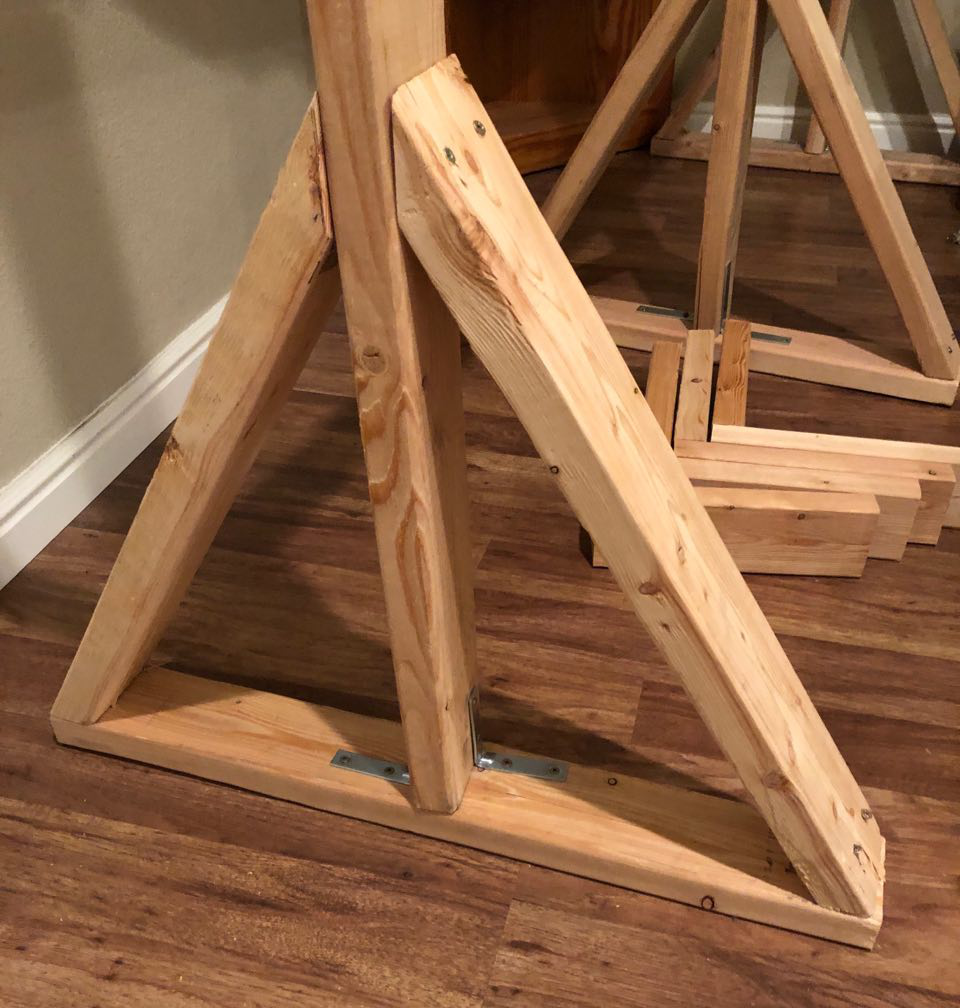
\includegraphics[width=0.5\textwidth]{image5.png}
  \caption{Triangle stand for holding the 3D LED Canvas.}
  \label{fig:framelegs}
\end{figure}

The frame was still needing a way to stand on it owns. The easiest and the fastest way to hold the frame standing was to create triangle supports as seen in Fig. \ref{fig:framelegs}. Triangles prevent the frame from tilting forward or backward since the art piece is top heavy. We added triangle supports to all three legs. We were pleased with the outcome of this frame.

To attach the LEDs on front of this frame, we added supports on the left, right and the top. The LED strips were first mounted on to a normal bed sheet with a hot glue gun. This bed sheet was then mounted on the front of the frame. Another white sheet was mounted on top the LED strips (sandwiching the LED strips between the two sheets) to create a clean white canvas.

Finally, we mounted all of the power supplies on the back of the frame. We also mounted our microcontroller unit with the PCB on the back. The wiring for all 18 LED strips along with the wiring for the stepper motor was getting a bit messy. To clean this up, we used some wire management hooks to organize the wires. After sanding out the sharp corners and cleaning few things up, our frame was complete.

\section{Evaluation}
During the planning phase, we wanted to make sure that the linear track system worked smoothly. The linear track system is one of the biggest parts of the art piece and if that didn’t work it would have made the art piece unacceptable. When assembling the linear tracks, we were surprised how well the aluminum extrusions worked. We did encounter a few problems during the assembly phase. However, these were minor problems such as screws being to long or the timing belt being too short. Another concern of ours was the weight of the Y-axis arm. We thought the weight of that arm would prevent it from moving smoothly. This concern was quickly dismissed once we mounted the linear track to the wood frame. There was also another problem with the arm and the joints of the two 1m extrusions (for the X-axis). We noticed that the arm was not passing through the joint smoothly. After sanding the joints, this problem was resolved. 

We may have gotten motors with too high of torque, which is not necessarily bad, but we did not take into account the weight of these motors. Interfacing with the stepper motors was a bit complicated. Early on, we noticed that stepping a motor was a blocking task which basically means that the rest of our program would pause while the motors were moving. This also meant we could only move one motor at a time. To solve this, we’re stepping each motor one a step at a time to make it seem like both of the motors are moving together. Other than that, the motors worked out great for us.

The LED strips we purchased also worked great. The strips were exactly what we were looking for. The arduino library made it easy to interface with, change colors, and index each LED individually. The only problem we encountered for the LED strips was related to power required to turn them all on. Since each strip needs 4A and we have 18 strips, we needed exactly 72A. However, we were never planning on using all the LED pixels all at once with full brightness so we didn’t need a 72A power supply.

Our plan from the beginning was to have the user interact with the canvas wirelessly. To achieve this, we used a Bluetooth module. We spent quite a bit of time interfacing with the Bluetooth module. The connection between the iOS app and the Bluetooth was poor and could not send all of the data fast enough. After tinkering around with it for a while, we ended up rewriting the Bluetooth controller (in arduino). This seemed to resolve the issue and we started to receive data from the iOS app much faster. Once the Bluetooth was working, controlling the motors and the LEDs was simple. We had already written code to control both of these locally, which meant adding wireless capability to it required slight change of code.

As for the iOS application itself, everything went fairly smoothly. The biggest hurdles for the application was writing new things in Swift that we were not familiar with. This main relatively simple tasks take quite a bit longer than expected since we had to learn as we went. The drawing portion of the application was relatively simple to implement using the CoreGraphics framework which is a drawing engine. The hardest challenge with the drawing part was getting the “paint” to fade so that when a user draws a line, the line begins to fade from the first drawn pixel to the most recently drawn pixel. This required us to implement our own generic Queue class since Swift 4 does not have its own Queue data structure. We chose to make the class generic so that we could use the Queue if we needed it for anything other than pixels. Figuring out how to get a generic class working in Swift proved to take a little more time than expected but now it works perfectly.

We use the Queue to store all of the lines that a user has drawn. A timer is set up within the controller that checks the Queue full of lines and begins to change the alpha values of each line. This gives us a trail-fading effect that we were aiming for from the start. Overall, using Swift was a great experience and gave us another tool to use in our toolbelts.

\section{Conclusion}
Ultimately, the project was a success. We accomplished the task we set out to do and we were able to showcase our computer engineering skills as a form of art. Our archive of the progress for this project can be found at magicdrawing.unityx.io. We took on some challenges that put us out of our comfort zone and proved that we could step to the challenge and succeed. Though our project was a success, we have also learned that we will always be confronted with some task that we may not know how to accomplish and we will have to learn how to adapt our existing knowledge to complete the task. We will always be learning and continuing our education throughout our careers.

\newpage

\begin{appendices}
  \section{Discoveries and Pitfalls}
  With having little to no background in mechanical engineering, we needed extensive research to get the linear track system moving. We learned a lot from doing the research. One suggestion we have for other groups is to make sure there is enough time to do the research and tinker with the mechanical components. We had a few problems that could have easily been avoided had we known how the mechanical parts worked.

  \section{Parts}
  \begin{longtable}{ p{5cm} p{10cm} }
    LED Pixel Strips             & \href{https://www.adafruit.com/product/1376?length=2}{18 x Adafruit NeoPixel Digital RGB LED Strip - 30 LED} \\[0.4cm]
    
    Bluetooth                    & \href{https://www.adafruit.com/product/2479}{1 x Adafruit Bluefruit LE UART Friend - Bluetooth Low Energy (BLE)} \\[0.4cm]
    
    Arduino                      & \href{https://store.arduino.cc/usa/arduino-mega-2560-rev3}{1 x Arduino Mega 2560 Rev 3} \\[0.4cm]
    
    Stepper Motors                & \href{https://openbuildspartstore.com/nema-23-stepper-motor-high-torque-series/}{2 × NEMA 23 Stepper Motor - High Torque Series} \\[0.4cm]

    Motor Drivers                & \href{https://www.pololu.com/product/2970}{2 x AMIS-30543 Stepper Motor Driver} \\[0.4cm]
    
    Linear Tracks (Gantry carts,
    timing belts, wheels, etc.)  & \href{https://openbuildspartstore.com/v-slot-20x80-linear-rail/}{1 x V-Slot 20x80 Linear Rail} \newline
    \href{https://openbuildspartstore.com/v-slot-20x60-linear-rail/}{4 x V-Slot 20x60 Linear Rail} \newline
    \href{https://openbuildspartstore.com/v-slot-20x40-linear-rail/}{3 x V-Slot 20x40 Linear Rail} \newline
    \href{https://openbuildspartstore.com/v-slot-gantry-set-universal/}{3 x V-Slot Gantry Set} \newline
    \href{https://openbuildspartstore.com/3gt-gt2-3m-timing-belt-by-the-foot/}{22ft 3GT (GT2-3M) Timing Belt} \newline
    \href{https://openbuildspartstore.com/3gt-timing-pulley-20-tooth/}{2 x 3GT (GT2-3M) Timing Pulley - 20 Tooth} \newline
    \href{https://openbuildspartstore.com/micro-limit-switch-kit/}{2 x Micro Limit Switch Kit} \newline6 x Eowpower 600V 25A Dual Row 8 Position Bus Bar     \\[0.4cm]
    
    Linear Actuator              & \href{https://openbuildspartstore.com/micro-limit-switch-kit/}{
Mini Linear Actuator} \\[0.4cm]
    
    Power Supplies               & \href{https://openbuildspartstore.com/24v-14-6a-meanwell-power-supply/}{1 x 24V/14.6A Meanwell Power Supply} \newline
    \href{https://www.amazon.com/Tanbaby-Universal-Regulated-Switching-Computer/dp/B017YEOAPA}{1 x Tanbaby 5V 60A DC Universal Regulated Switching Power Supply 300w} \newline
    \href{https://www.amazon.com/gp/product/B06XKFCTSM/ref=oh_aui_detailpage_o05_s00?ie=UTF8&psc=1}{6 x Eowpower 600V 25A Dual Row 8 Position Bus Bar } \\
    
    Miscellaneous                & Lumber (6 x 10ft 2x4) \newline
    Various screws, L-brackets, washers, etc. \newline
    Normal bed sheets for the canvas\\
  \end{longtable}
  
  \section{Schematics and Code}
  We used Github for all of our development. Our Github repository is \href{https://github.com/rajp20/LED_Canvas}{LED\_Canvas}. This repository contains all of our code for iOS app and the microcontroller firmware. 
\end{appendices}

\end{document}
